\subsection{Client}

\subsubsection{Architettura}
L'architettura del client è più semplice: effettua richieste in formato JSON e resta in attesa di una risposta. Il thread grafico è aggiornato all'occorrenza dal metodo \texttt{invokeLater}. Durante la normale esecuzione, il client è single threaded; viene generato al bisogno un thread per la ricezione di messaggi multicast, durante la modifica di un documento.

\medskip

L'interfaccia grafica si adatta automaticamente alle dimensioni dello scher\-mo, ed è stato cercato di renderla il più coerente e intuitiva possibile.

\medskip

Dalla schemata di registrazione e login si può accedere all'area personale di \texttt{TURING}, dove ogni utente può creare nuovi documenti, invitare altri utenti alla modifica, e in una tabella dinamica vede i documenti che può modificare, con la lista delle sezioni e informazioni aggiuntive, come il nome del creatore del documento (indispensabile nel caso di documenti omonimi) e un'icona che indica se il documento è stato condiviso o no. La tabella si aggiorna in tempo reale quando si viene invitati alla modifica di un nuovo documento (con apposito messaggio di notifica), ma è anche possibile forzare un aggiornamento manuale tramite il tasto ``refresh".

\medskip

Dopo che una sezione di un documento è stata selezionata per la modifica, viene visualizzata la schermata di lavoro, nella quale è possibile modificare il testo precedentemente salvato, chattare con gli utenti che stanno modificando lo stesso documento, salvare le modifiche o ignorarle.

\begin{center}
	\begin{figure}[ht!]
		\makebox[\textwidth]{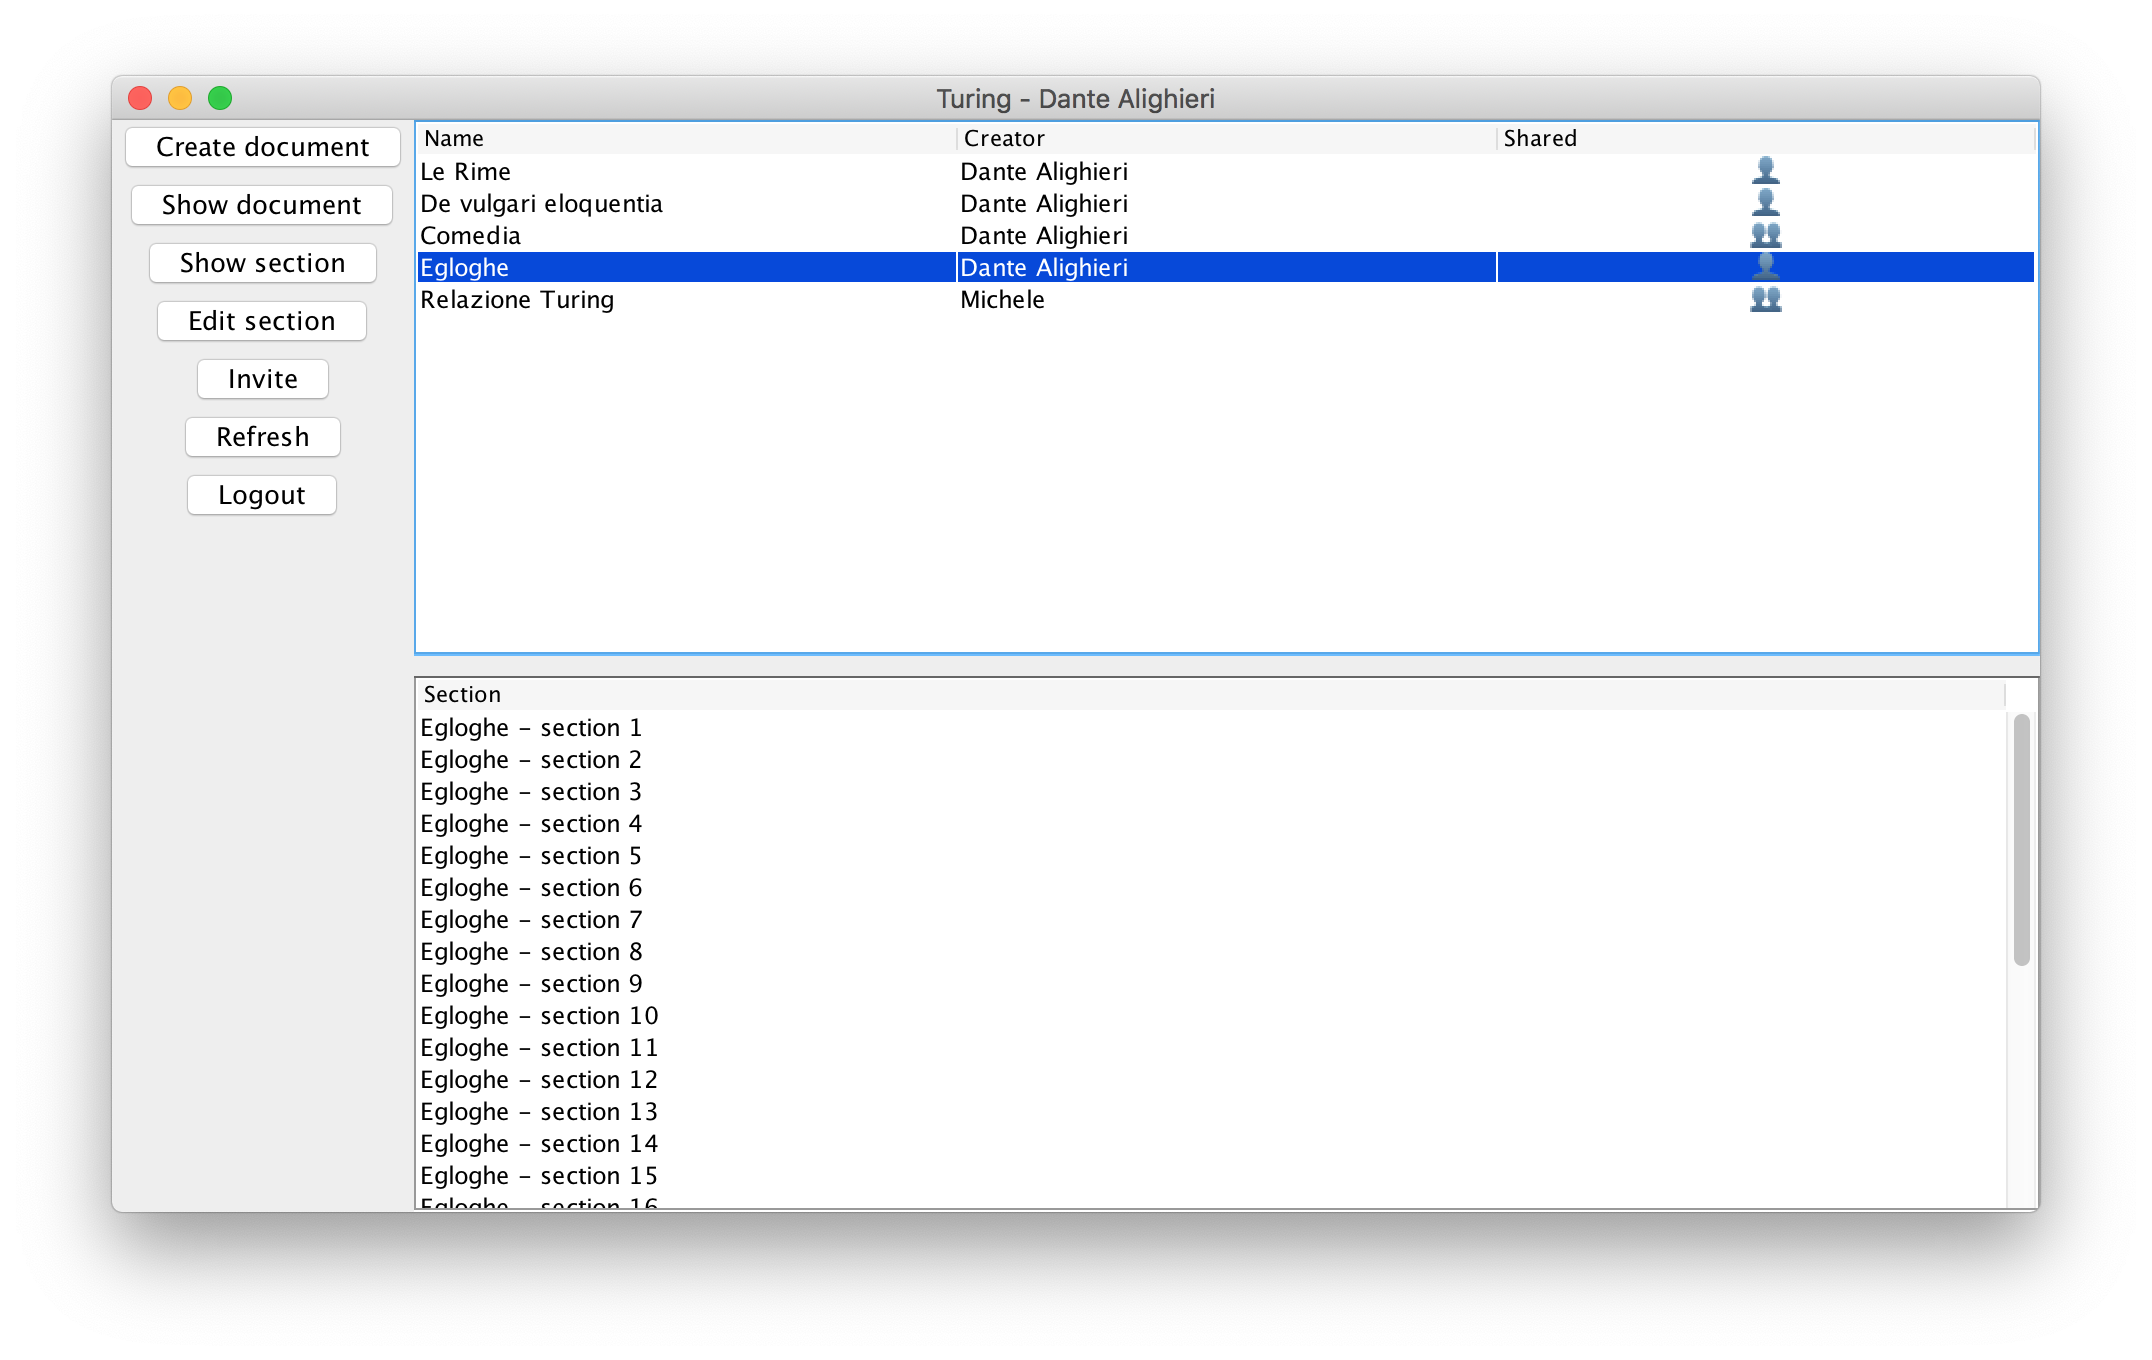
\includegraphics[width=1.4\linewidth]{screenshots/documents.png}}
		\caption{Elenco dei documenti di Dante Alighieri. Notare le icone per indicare la condivisione o meno di un documento.}
	\end{figure}

	\begin{figure}[ht!]
		\makebox[\textwidth]{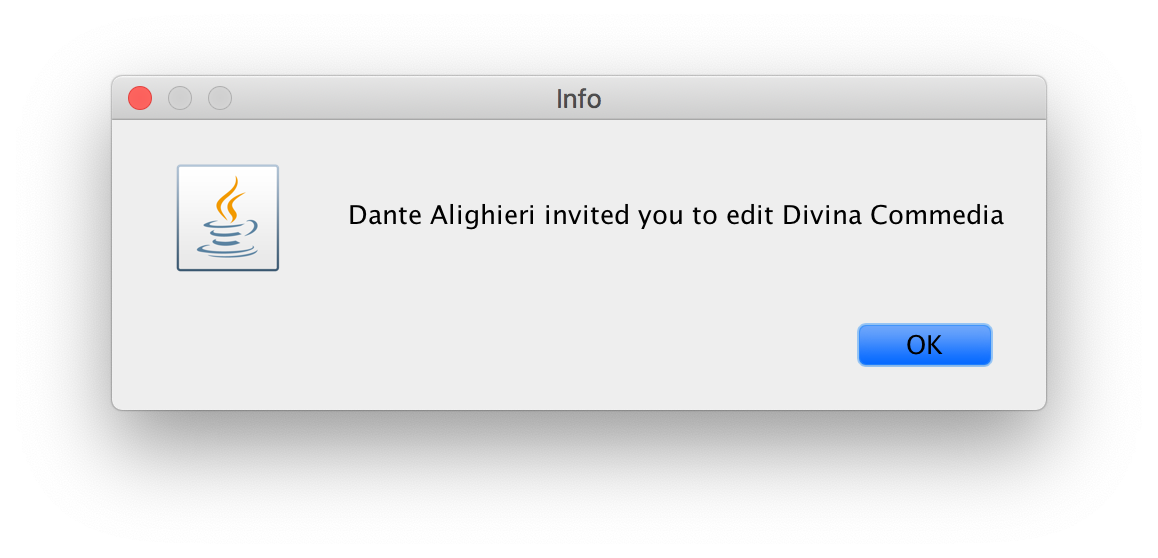
\includegraphics[width=0.70\linewidth]{screenshots/notification.png}}
		\caption{Notifica che indica che Michele è stato invitato alla modifica della Divina Commedia da parte di Dante Alighieri.}
	\end{figure}

	\begin{figure}[ht!]
		\makebox[\textwidth]{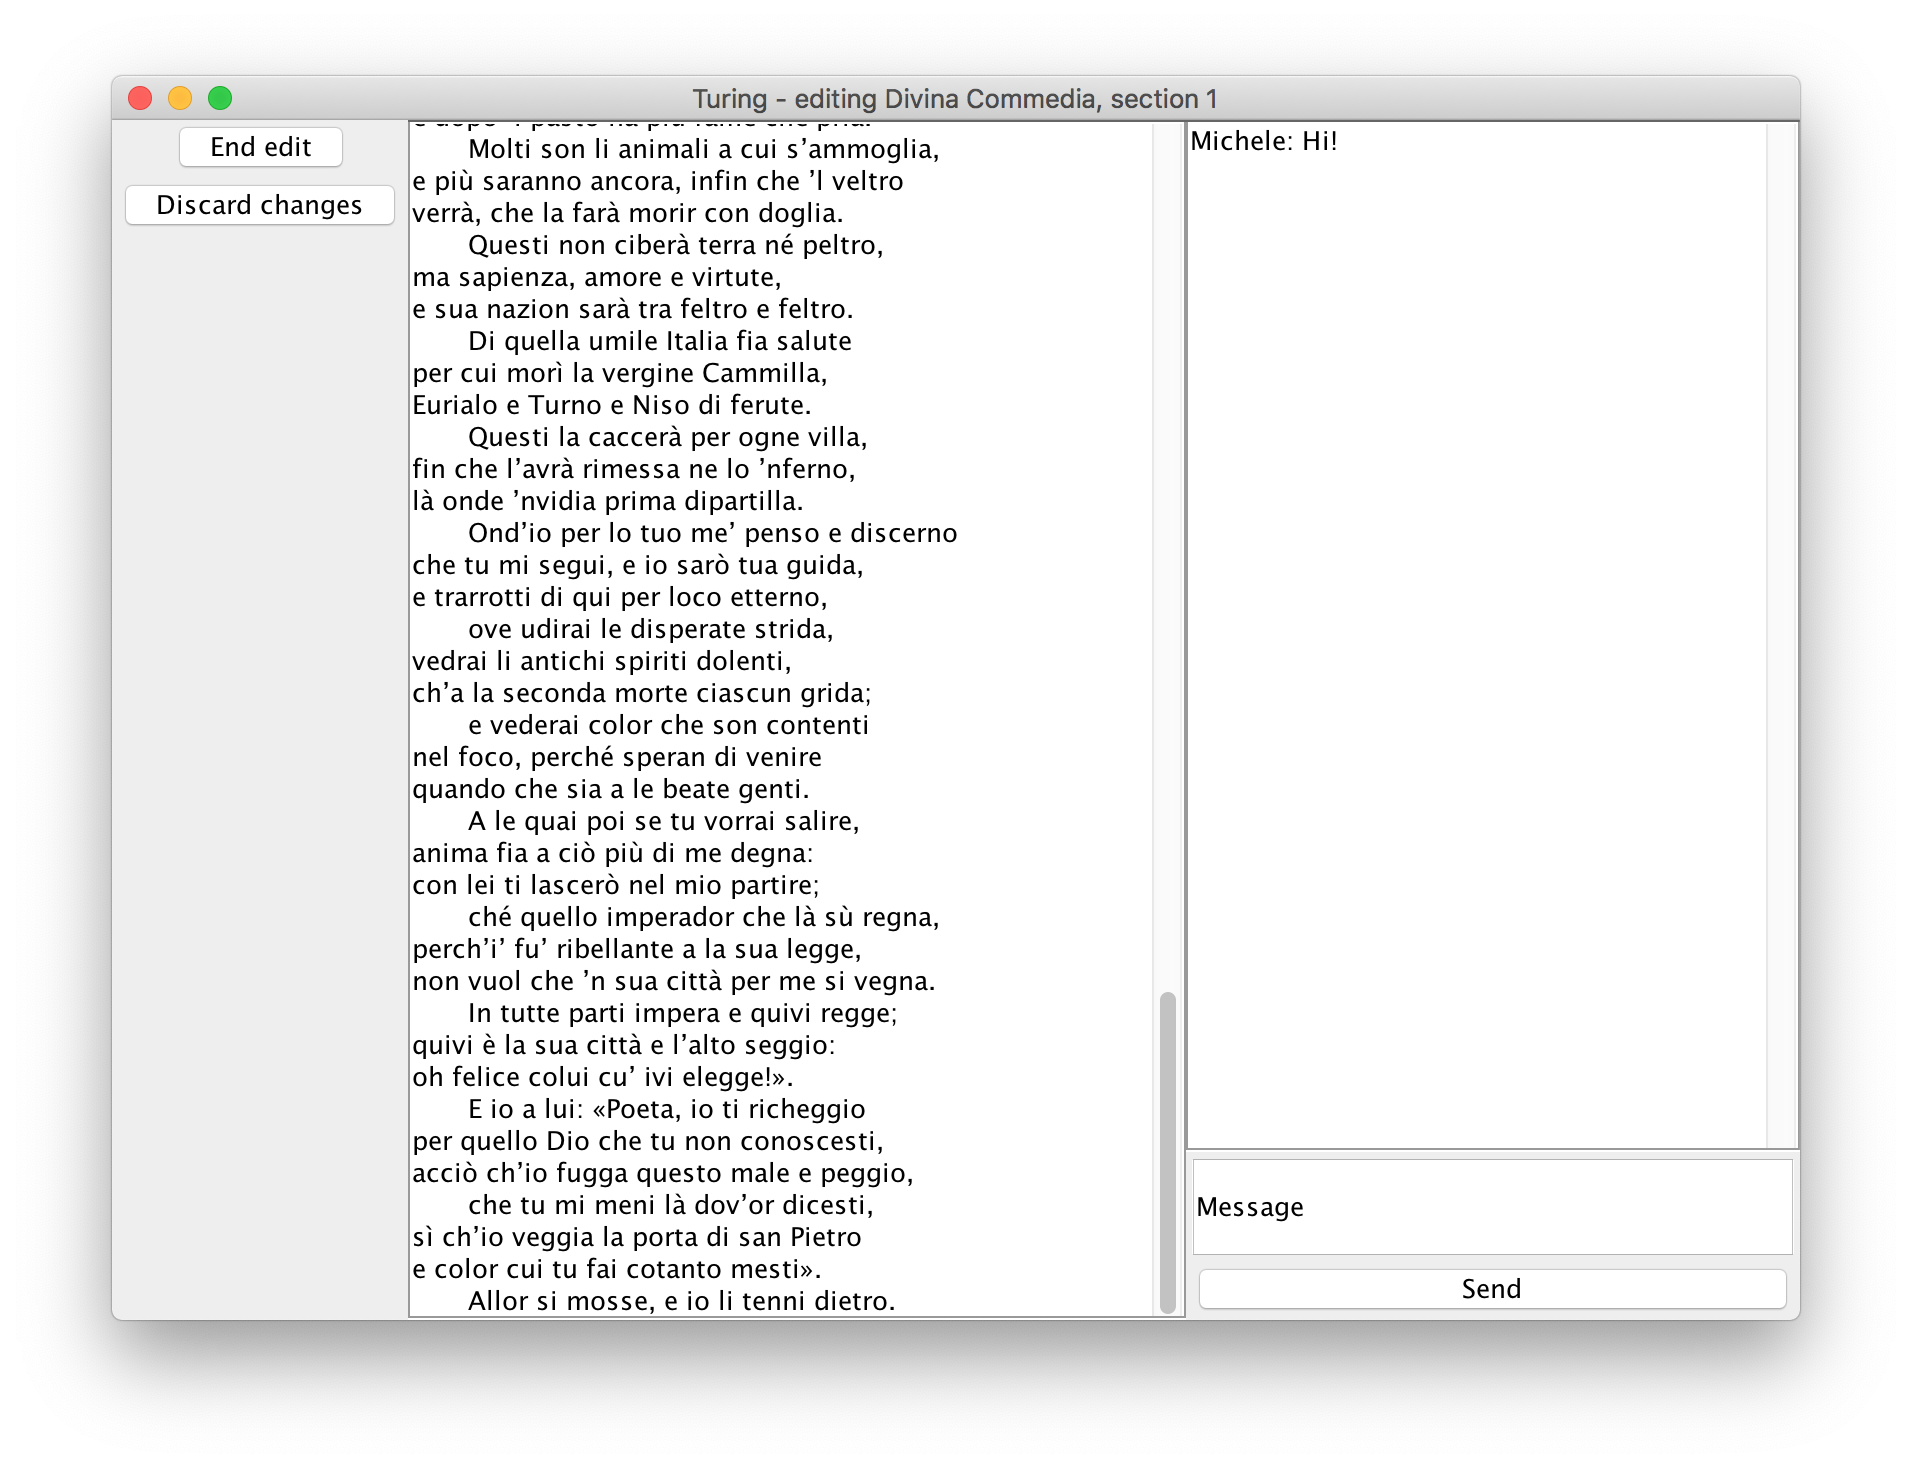
\includegraphics[width=1.20\linewidth]{screenshots/workspace.png}}
		\caption{Dante Alighieri modifica la prima sezione della Divina Commedia, mentre gli arriva un messaggio in chat da Michele.}
	\end{figure}
\end{center}

\newpage
